\begin{abstract}
This document contains the solution of geometry through linear algebra through the concept of optimization.
\end{abstract}
Download latex and python codes from 
\begin{lstlisting}
https://github.com/sahilsin/AI_ML/blob/master/Assignment3/
\end{lstlisting}
%
\section{Problem}
Minimize and Maximize $Z=5x+10y$ subject to $x+2y\leq120$, $x+y\geq60$, $x-2y\geq0$, $x,y\geq0$.\\
\section{Solution}

First we will plot these lines which are the constraints and the area enclosed by is the region we are interested in.

\begin{figure}[h]
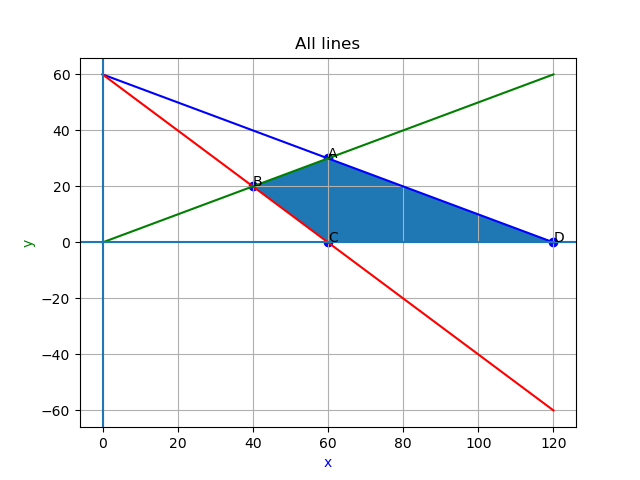
\includegraphics[width=\columnwidth]{figs/Figure_1.png}
\caption{optimal point through the intersection of various lines}
\label{fig:Figure_1}
\end{figure}

The four points are the points which will maximize and minimize the function.These corner points are :
\begin{align*}
    A=(60,30)
\\
    B=(40,20)
\\
    C=(60,0)
\\
    D=(120,0)
\end{align*}

Value of Z at point

\begin{align*}
     A= 5\times 60 + 10 \times 30 =600
\\
     B= 5\times 40 + 10 \times 20 =400
\\
     C= 5\times 60 + 10 \times 0 =300
\\
     D= 5\times 120 + 10 \times 0 =600
\end{align*}

We can see that our function Z is maximum at points A and D that is (60,30) and (120,0)\\
and\\
Z is minimum at point C that is (60,0)\\
%
\section{Verification}
The given solution can be verified through the given code.\\
The given problem can be solved using {\em pulp} through the following code
\begin{lstlisting}
https://github.com/sahilsin/AI_ML/blob/master/Assignment3/codes/Ai_ML_3.py
\end{lstlisting}
